\documentclass[epsfig,10pt,fullpage]{article}

\newcommand{\LabNum}{9}
\newcommand{\CommonDocsPath}{../../../common/docs}
\addtolength{\textwidth}{1.5in}
\addtolength{\oddsidemargin}{-0.75in}
\addtolength{\topmargin}{-0.75in}
\addtolength{\textheight}{1.5in}
\addtolength{\evensidemargin}{0.75in}
\setlength\parindent{0pt}
\raggedbottom

\usepackage{ae,aecompl}
\usepackage{epsfig,float,times}
\usepackage[hypcap]{caption}
\usepackage[pdftex, colorlinks]{hyperref}
\usepackage{graphicx}
\usepackage[usenames, dvipsnames]{color}
\usepackage{rotating}
\usepackage{tikz}
\usetikzlibrary{automata,positioning}
\usepackage{placeins}

\widowpenalty 10000
\clubpenalty 10000

\newcommand{\red}[1]{{\color{red}\sf{#1}}}
\newcommand{\green}[1]{{\color{green}\sf{#1}}}
\newcommand{\blue}[1]{{\color{blue}\sf{#1}}}
\definecolor{PineGreen}{rgb}{0.0, 0.47, 0.44}
\definecolor{ForestGreen}{rgb}{0.13, 0.55, 0.13}
\definecolor{Brown}{rgb}{0.59, 0.29, 0.0}

\newcommand{\UPDatePublished}{Oct 2021}
\newcommand{\versnum}{21.1} %version number quartus/AMP
\newcommand{\quartusname}{Quartus\textsuperscript{\textregistered} Prime}	
\newcommand{\UPTextBar}{For \quartusname{} \versnum{}}
\newcommand{\thisyear}{2021 } %for copyright
\newcommand{\company}{FPGAcademy.org}
\newcommand{\longteamname}{FPGAcademy.org}
\newcommand{\teamname}{FPGAcademy}
\newcommand{\website}{FPGAcademy.org}

\newcommand{\productAcronym}{AMP}
\newcommand{\productNameShort}{Monitor Program}

\newcommand{\productNameMedTM}{A Monitor Program}
\newcommand{\productNameMed}{A Monitor Program}

%\newcommand{\headerLogoFilePath}[1]{#1/FPGAcademy.png}

% listings is a package that supports encapsulating source code in LaTeX conveniently
\usepackage{listings}

\def\expandparam\lstinputlisting[#1]#2{\edef\tmp{\noexpand\lstinputlisting[#1]{#2}}\tmp}

%%%%%%%%%%%%%%%%%%%% Source Code Formatting %%%%%%%%%%%%%%%%%%%%
\definecolor{globalCommentColour}{rgb}{0.588,0.588,0.588}

%%%%%%%%%%%%%%%%%%%%%%%%%%%%%%%%%%%%%%%%%%%%%%%%%%%%
% Defining language style
% NiosII ASM
\lstdefinelanguage[NiosII]{Assembler} {
  morekeywords={add, addi, and, andhi, andi, beq, bge, bgeu, bgt, bgtu, ble,  bleu, blt, bltu, bne, br, break,
  bret, call, callr, cmpeq, cmpeqi, cmpge, cmpgei, cmpgeu, cmpgeui, cmpgt, cmpgti, cmpgtu, cmpgtui, cmple,
  cmplei, cmpleu, cmpleui, cmplt, cmplti, cmpltu, cmpltui, cmpne, cmpnei, custom, div, divu, eret, flushd,
  flushda, flushi, flushp, initd, initda, initi, jmp, jmpi, ldb, ldbio, ldbu, ldbuio, ldh, ldhio, ldhu, ldhuio,
  ldw, ldwio, mov, movhi, movi, movia, movui, mul, muli, mulxss, mulxsu, mulxuu, nextpc, nop, nor, or, orhi, ori,
  rdctl, rdprs, ret, rol, roli, ror, sll, slli, sra, srai, srl, srli, stb, stbio, sth, sthio, stw, stwio,
  sub, subi, sync, trap, wrctl, wrtcl, wrprs, xor, xori, xorhi, xori},
  morekeywords=[2]{.abort, .ABORT, .align, .app-file, .ascii, .asciz, .balign, .byte, .comm, .data, .def,
  .desc, .dim, .double, .eject, .else, .end, .endef, .endif, .equ, .equiv, .err, .extern, .file, .fill, .float,
  .global, .globl, .hword, .ident, .if, .include, .int, .irp, .irpc, .lcomm, .lflags, .line, .linkonce, .ln,
  .list, .long, .macro, .mri, .nolist, .octa, .org, .p2align, .psize, .quad, .rept, .sbttl, .scl, .section,
  .set, .short, .single, .size, .sleb128, .skip, .space, .stadb, .stabn, .stabs, .string, .symver, .tag,
  .text, .title, .type, .val, .uleb128, .word},
  morekeywords=[3]{et, bt, gp, sp, fp, ea, sstatus, ra, pc, status, estatus, bstatus, ienable, ipending, cpuid,
  exception, pteaddr, tlbacc, tlbmisc, eccinj, badaddr, config, mpubase, mpuacc},
  sensitive=t,
  alsoletter=.,
  morestring=[b]",
  morecomment=[s]{/*}{*/},
  morecomment=[l]\#,
}[keywords,comments,strings]
   
%% NOTE: morekeywords=[2] are GNU directives.
   
\definecolor{niosInstructionColour}{rgb}{0.000,0.608,0.000}
\definecolor{niosDirectiveColour}{rgb}{0.000,0.000,0.902}
\definecolor{niosSpecialRegColour}{rgb}{0.000,0.000,0.000}
\definecolor{niosStringColour}{rgb}{0.808,0.482,0.000}
   
%% NOTE: To make bold use: =\bfseries\color{<colour>}
\lstdefinestyle{defaultNiosStyle} {
  language=[NiosII]{Assembler},
  stringstyle=\color{niosStringColour},
  keywordstyle=\color{niosInstructionColour},
  keywordstyle=[2]\color{niosDirectiveColour},
  keywordstyle=[3]\itshape\color{niosSpecialRegColour}
}
%%%%%%%%%%%%%%%%%%%%%%%%%%%%%%%%%%%%%%%%%%%%%%%%%%%%

%%%%%%%%%%%%%%%%%%%%%%%%%%%%%%%%%%%%%%%%%%%%%%%%%%%%
% Defining language style
% ArmA9 ASM
\lstdefinelanguage[ArmA9]{Assembler} {
  morekeywords={ADC, ADD, ADDS, AND, ANDS, B, BAL, BEQ, BGE, BGT, BL, BLT, BIC, BKPT, BLX, BNE, BX, CDP, CLZ, CMN, CMP, EOR,
  EORS, LDC, LDM, LDR, LDRB, LDRBT, LDRH, LDRSB, LDRSH, LDRT, LSL, MCR, MLA, MOV, MOVW, MOVT, MRC, MRS, MSR, MUL, MVN, ORR, PLD,
  ROR, RSB, RSC, SBC, SMLAL, SMULL, STC, STM, STR, STRB, STRBT, STRH, STRT, SUB, SUBS, SWI, SWP, SWPB, TEQ, UMLAL,
  PUSH, POP, MOVS, RORS, LSR},
  morekeywords=[2]{.abort, .ABORT, .align, .app-file, .ascii, .asciz, .balign, .byte, .comm, .data, .def,
  .desc, .dim, .double, .eject, .else, .end, .endef, .endif, .equ, .equiv, .err, .extern, .file, .fill, .float,
  .global, .globl, .hword, .ident, .if, .include, .int, .irp, .irpc, .lcomm, .lflags, .line, .linkonce, .ln,
  .list, .long, .macro, .mri, .nolist, .octa, .org, .p2align, .psize, .quad, .rept, .sbttl, .scl, .section,
  .set, .short, .single, .size, .sleb128, .skip, .space, .stadb, .stabn, .stabs, .string, .symver, .tag,
  .text, .title, .type, .val, .vectors, .uleb128, .word},
  morekeywords=[3]{SP, PC, MIDR, CTR, TCMTR, TLBTR, MPIDR, ID_PFR0, ID_PFR1, ID_DFR0, ID_MMFR0, ID_MMFR1, ID_MMFR2,
  ID_MMFR3, ID_ISAR0, ID_ISAR1, ID_ISAR2, ID_ISAR3, ID_ISAR4, CCSIDR, CLIDR, AIDR, CSSELR, TTBR0, TTRB1, TTBR2, DACR,
  DFSR, IFSR, ADFSR, AIFSR, DFAAR, IFAR, ICIALLUIS, BPIALLIS, PAR, ICIALLU, ICIMVAU, BPIALL, DCIMVAC, DCISW, V2PCWPR,
  DCCVAC, DCCSW, DDIMVAC, DCISW, TLBALLIS, TLBIMVAIS, TLBIASIDIS, TLBIMVAAIS, TLBIALL, TLBIMVA, TLBIASID, TLBIMVAA,
  PMCR, PMCNTENSET, PMCNTENCLR, PMOVSR, PMSWINC, PMSELR, PMXEVTYPER, PMXEVCNTR, PMUSERENR, PMINTENSET, PMINTENCLR,
  PRRR, NRRR, PLEIDR, PLEASR, PLEFSR, PLEUAR, PLEPCR, VBAR, MVBAR, ISR, FCSEIDR, CONTEXTIDR, TPIDRURW, TPIDRURO, TPIDRPRW},
  sensitive=f,
  alsoletter=.,
  morestring=[b]",
  morecomment=[s]{/*}{*/},
  morecomment=[l]{//},
}[keywords,comments,strings]
   
%% NOTE: morekeywords=[2] are GNU directives.
   
\definecolor{armInstructionColour}{rgb}{0.000,0.608,0.000}
\definecolor{armDirectiveColour}{rgb}{0.000,0.000,0.902}
\definecolor{armSpecialRegColour}{rgb}{0.000,0.000,0.000}
\definecolor{armStringColour}{rgb}{0.808,0.482,0.000}
   
\lstdefinestyle{defaultArmStyle} {
  language=[ArmA9]{Assembler},
  stringstyle=\color{armStringColour},
  keywordstyle=\color{armInstructionColour},
  keywordstyle=[2]\color{armDirectiveColour},
  keywordstyle=[3]\itshape\color{armSpecialRegColour}
}
%%%%%%%%%%%%%%%%%%%%%%%%%%%%%%%%%%%%%%%%%%%%%%%%%%%%

%%%%%%%%%%%%%%%%%%%%%%%%%%%%%%%%%%%%%%%%%%%%%%%%%%%%
% Defining language style
% FPGAcademy ASM
\lstdefinelanguage{ASM}{
  morekeywords = [1]{mv, mvt, mvne, mvcc, add, sub, st, ld, and, b, bne, beq, bcc, bcs},
  morekeywords = [2]{word, define},
  keywordstyle = [1]\color{ForestGreen},
  keywordstyle = [2]\color{blue},
  sensitive = true,
  morecomment = [l]{//},
}

\lstset{
  language = ASM,
  basicstyle=\small\color{black}\ttfamily,
  commentstyle=\small\color{Brown}\itshape\ttfamily,
  showstringspaces=false,
  frame=none, %lines % boxed listings
  breaklines=true,
  breakatwhitespace=true,
  tabsize=3
}
%%%%%%%%%%%%%%%%%%%%%%%%%%%%%%%%%%%%%%%%%%%%%%%%%%%%

%%%%%%%%%%%%%%%%%%%%%%%%%%%%%%%%%%%%%%%%%%%%%%%%%%%%
% Defining language style
% Java
\definecolor{javaStringColour}{rgb}{0.808,0.482,0}
%%%%%%%%%%%%%%%%%%%%%%%%%%%%%%%%%%%%%%%%%%%%%%%%%%%%

%%%%%%%%%%%%%%%%%%%%%%%%%%%%%%%%%%%%%%%%%%%%%%%%%%%%
% Defining language style
% C
\definecolor{CStringColour}{rgb}{0.808,0.482,0}

\lstset{
  language = C,
  basicstyle=\small\color{black}\ttfamily, 
  commentstyle=\small\color{PineGreen}\itshape\ttfamily,
  keywordstyle=\small\color{blue}\bfseries\ttfamily,
  showstringspaces=false,
  frame=none, %lines % boxed listings
  breaklines=true,
  breakatwhitespace=true,
  tabsize=3
}
%%%%%%%%%%%%%%%%%%%%%%%%%%%%%%%%%%%%%%%%%%%%%%%%%%%%

%%%%%%%%%%%%%%%%%%%%%%%%%%%%%%%%%%%%%%%%%%%%%%%%%%%%
% Defining language style
% Verilog
\definecolor{verilogCommentColour}{rgb}{0.000,0.502,0.000}

\lstdefinestyle{defaultVerilogStyle} {
  language={Verilog},
  keywordstyle=\color{blue},
  commentstyle=\color{verilogCommentColour}
}
%%%%%%%%%%%%%%%%%%%%%%%%%%%%%%%%%%%%%%%%%%%%%%%%%%%%

%%%%%%%%%%%%%%%%%%%%%%%%%%%%%%%%%%%%%%%%%%%%%%%%%%%%
% Defining language style
% VHDL
\lstdefinestyle{defaultVHDLStyle} {
  language={VHDL},
  keywordstyle=\color{blue},
  commentstyle=\color{verilogCommentColour}
}
%%%%%%%%%%%%%%%%%%%%%%%%%%%%%%%%%%%%%%%%%%%%%%%%%%%%

%%%%%%%%%%%%%%%%%%%%%%%%%%%%%%%%%%%%%%%%%%%%%%%%%%%%
% Defining language style
% LaTeX
\lstdefinelanguage[LocalLaTeX]{TeX}[LaTeX]{TeX}{moretexcs={bf, it, sf, lstset},}

\lstdefinestyle{defaultLocalLatexStyle} {
  language=[LocalLatex]{TeX},
  keywordstyle=\color{blue}\bfseries,
  keywordstyle=[2]\color{blue},
  keywordstyle=[3]\color{blue}\bfseries
}
%%%%%%%%%%%%%%%%%%%%%%%%%%%%%%%%%%%%%%%%%%%%%%%%%%%%

%%%%%%%%%%%%%%%%%%%%%%%%%%%%%%%%%%%%%%%%%%%%%%%%%%%%
% Defining language style
% Default
\lstset{
  basicstyle=\small\color{black}\ttfamily,
  commentstyle=\small\color{globalCommentColour}\itshape\ttfamily,
  keywordstyle=\small\color{blue}\bfseries\ttfamily,
  showstringspaces=false,
  frame=none, %lines % boxed listings
  breaklines=true,
  breakatwhitespace=true,
  tabsize=3
}
%%%%%%%%%%%%%%%%%%%%%%%%%%%%%%%%%%%%%%%%%%%%%%%%%%%%


\hypersetup{
  pdftitle={Digital Logic Lab Exercise \LabNum},
  linkcolor=blue,
  hyperindex=true,
  pdfauthor={FPGAcademy.org},
  pdfkeywords={FPGAcademy.org, FPGAcademy, Lab, Exercise, Digital Logic},
  bookmarks,
  bookmarksopen=false,
  filecolor=blue,
  pdfstartview={FitH},
  urlcolor=blue,
  plainpages=false,
  pdfpagelabels=true,
  linkbordercolor={1 1 1} %no color for link border
}



\begin{document}

\centerline{\huge Digital Logic}
~\\
\centerline{\huge Laboratory Exercise \LabNum}
~\\
\centerline{\large A Simple Processor}
~\\

Figure~\ref{fig:fig1} shows a digital system that contains a number of 16-bit registers,
a multiplexer, an adder/subtracter, and a control unit (finite state machine).  Information
is input to this system via the 16-bit {\it DIN} input, which is loaded into the {\it IR} 
register. Data can be transferred through the 16-bit wide multiplexer from one register
in the system to another, such as from register {\it IR} into one of the {\it general 
purpose} registers $r0, \ldots, r7$.  The multiplexer's output is called {\it Buswires} 
in the figure because the term {\it bus} is often used for wiring that allows data to be 
transferred from one location in a system to another. The FSM controls the {\it Select} 
lines of the multiplexer, which allows any of its inputs to be transferred to any register
that is connected to the bus wires.

~\\
The system can perform different operations in each clock cycle, as governed by the FSM. 
It determines when particular data is placed onto the bus wires and controls which of the 
registers is to be loaded with this data. For example, if the FSM selects $r0$ as the output of the 
bus multiplexer and also asserts $A_{in}$, then the contents of register $r0$ will be loaded on the 
next active clock edge into register {\it A}.

~\\
Addition or subtraction of signed numbers is performed by using the multiplexer to first 
place one 16-bit number onto the bus wires, and then loading this number into register {\it A}. 
Once this is done, a second 16-bit number is placed onto the bus, the adder/subtracter
performs the required operation, and the result is loaded into register {\it G}. The
data in {\it G} can then be transferred via the multiplexer to one of the other registers,
as required.

\begin{figure}[H]
	\begin{center}
		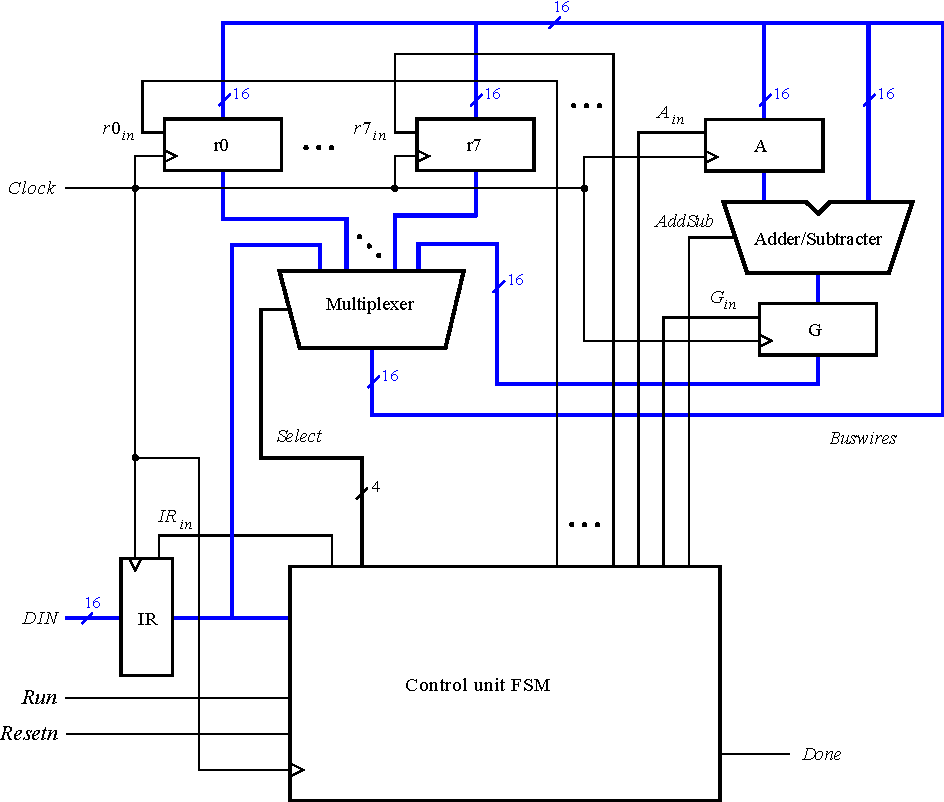
\includegraphics[scale = 0.8]{figures/figure1.pdf}
	\end{center}
	\caption{A digital system.}
	\label{fig:fig1}
\end{figure}

\newpage
\noindent
A system like the one in Figure~\ref{fig:fig1} is often called a {\it processor}. It 
executes operations specified in the 
form of {\it instructions}. Table~\ref{tab:instructions} lists the instructions that this 
processor supports. The left column shows the name of an instruction and its operands. 
The meaning of the syntax {\it rX} $\leftarrow$ {\it Op2} is that the second operand,
{\it Op2}, is loaded into register {\it rX}. The operand {\it Op2} can be either a
register, {\it rY}, or {\it immediate data}, \#{\it D}.

\begin{table}[H]
\begin{center}
\begin{tabular}{rl|c}
   \multicolumn{2}{c|}{Instruction} & Function performed \\ \hline 
   \rule[0.01in]{0in}{0.15in}{\it mv} & {\it rX}, $Op2$ & {\it rX} $\leftarrow Op2$ \\ 
		  \rule[-0.075in]{0in}{0.2in}{\it mvt} & {\it rX,} \#{\it D} & {\it rX$_{15-8}$} $\leftarrow$ {\it D$_{15-8}$}\\ 
   \rule[-0.075in]{0in}{0.2in}{\it add} & {\it rX}, $Op2$ & {\it rX} $\leftarrow$ {\it rX} + $Op2$ \\ 
   \rule[-0.075in]{0in}{0.2in}{\it sub} & {\it rX}, $Op2$ & {\it rX} $\leftarrow$ {\it rX} $-$ $Op2$ \\ 
\end{tabular}
\caption{Instructions performed in the processor.}
\label{tab:instructions}
\end{center}
\end{table}

\noindent
Instructions are loaded from the external input {\it DIN}, and stored into the {\it IR} register, 
using the connection indicated in Figure~\ref{fig:fig1}. Each instruction is {\it encoded} using 
a 16-bit format. If $Op2$ specifies a register, then the instruction encoding is 
\texttt{III0XXX000000YYY}, where \texttt{III} specifies the instruction, \texttt{XXX} gives 
the {\it rX} register, and \texttt{YYY} gives the {\it rY} register. If $Op2$ specifies 
immediate data \#{\it D}, then the encoding is 
\texttt{III1XXXDDDDDDDDD}, where the 9-bit field \texttt{DDDDDDDDD} represents the constant data.
Although only two bits are needed to encode our four instructions, we are using three bits because 
other instructions will be added to the processor later. Assume that \texttt{III} $= 000$ for
the {\it mv} instruction, $001$ for {\it mvt}, $010$ for {\it add}, and $011$ for {\it sub}. 

~\\
The {\it mv} instruction ({\it move}) copies the contents of one register into 
another, using the syntax \texttt{mv} \texttt{rX,rY}. It can also be used to initialize a 
register with immediate data, as in \texttt{mv} \texttt{rX,\#D}.  Since the data {\it D} 
is represented inside the encoded instruction using only nine bits, the processor has to 
{\it zero-extend} the data, as in \texttt{0000000D$_{8-0}$}, before loading it into 
register~{\it rX}.  The {\it mvt} instruction ({\it move top}) is used to initialize the 
most-significant byte of a register.  For {\it mvt}, only eight bits of the {\it D} field in 
the instruction are used, so that \texttt{mvt} \texttt{rX,\#D} loads the value 
\texttt{D$_{15-8}$00000000} into {\it rX}. As an example, to load register $r0$ with the 
value \texttt{0xFF00}, you would use the instruction \texttt{mvt r0,\#0xFF00}.  The instruction 
\texttt{add} \texttt{rX,rY} produces the sum {\it rX} $+$ {\it rY} and loads the result 
into {\it rX}. The instruction \texttt{add} \texttt{rX,\#D} produces the 
sum {\it rX} $+$ {\it D}, where {\it D} is zero-extended to 16 bits, and saves the result 
in {\it rX}. Similarly, the {\it sub} instruction generates 
either {\it rX} $-$ {\it rY}, or {\it rX} $-$ \#{\it D} and loads the result into {\it rX}.

~\\
Some instructions, such as an {\it add} or {\it sub}, take a few clock cycles to complete, 
because multiple transfers have to be performed across the bus. The finite state machine in the 
processor ``steps through'' such instructions, asserting the control signals needed in 
successive clock cycles until the instruction has completed.  The processor starts executing 
the instruction on the {\it DIN} input when the {\it Run} signal is asserted and the processor 
asserts the {\it Done} output when the instruction is finished.  Table~\ref{tab:control_signals}
indicates the control signals from Figure~\ref{fig:fig1} that have to be 
asserted in each time step to implement the instructions in Table~\ref{tab:instructions}.  The 
only control signal asserted in time step $T_0$, for all instructions, is {\it IR}$_{in}$. 
The meaning of {\it Select = rY} or {\it IR} in the table is that the multiplexer selects 
either register {\it rY} or the immediate data in {\it IR}, depending on the value of $Op2$.
For the {\it mv} instruction, when {\it IR} is selected the multiplexer outputs 
\texttt{0000000DDDDDDDDD}, and for {\it mvt} the multiplexer outputs \texttt{DDDDDDDD00000000}.
Only signals from Figure~\ref{fig:fig1} that have to be asserted in each time 
step are listed in Table~\ref{tab:instructions}; all other signals are not asserted. The 
meaning of {\it AddSub} in step $T_2$ of the {\it sub} instruction is that this signal is set 
to 1, and this setting causes the adder/subtracter unit to perform subtraction using 
2's-complement arithmetic.

~\\
The processor in Figure~\ref{fig:fig1} can perform various tasks by using a sequence of 
instructions. For example, the sequence below loads the number 28 into register $r0$ and then 
calculates, in register $r1$, the 2's complement value $-28$.

\begin{minipage}[t]{15 cm}
\begin{lstlisting}
       mv    r0, #28        // original number = 28
       mvt   r1, #0xFF00
       add   r1, #0x00FF    // r1 = 0xFFFF
       sub   r1, r0         // r1 = 1's-complement of r0
       add   r1, #1         // r1 = 2's-complement of r0 = -28
\end{lstlisting}
\end{minipage}

\begin{table}[H]
\begin{center}
\begin{tabular}{r|c|c|c|c|}
\multicolumn{1}{c}{~} & \multicolumn{1}{c}{$T_0$} & \multicolumn{1}{c}{$T_1$} & \multicolumn{1}{c}{$T_2$} & \multicolumn{1}{c}{$T_3$} \rule[-0.075in]{0in}{0.25in}\\ \cline{2-5}
{\it mv~} & {\it IR}$_{in}$ & \rule[-0.075in]{0in}{0.25in}{\it Select} = {\it rY} or {\it IR}, &  &  \\
~ & ~ & {\it rX$_{in}$}, {\it Done} &  &  \\ \cline{2-5}
{\it mvt~} & {\it IR}$_{in}$ & \rule[-0.075in]{0in}{0.25in}{\it Select} = {\it IR}, &  &  \\
~ & ~ & {\it rX$_{in}$}, {\it Done} &  &  \\ \cline{2-5}
\rule[-0.075in]{0in}{0.25in}{\it add~} & {\it IR}$_{in}$ & {\it Select} = {\it rX}, & {\it Select} = {\it rY} or {\it IR}, & {\it Select = G}, {\it rX$_{in}$}, \\
~ & ~ & {\it A$_{in}$} &  {\it G$_{in}$} & {\it Done} \\
\cline{2-5}
\rule[-0.075in]{0in}{0.25in}{\it sub~} & {\it IR}$_{in}$ & {\it Select} = {\it rX}, & {\it Select} = {\it rY} or {\it IR}, & {\it Select = G}, {\it rX$_{in}$}, \\
~ & ~ & {\it A$_{in}$} &  {\it AddSub}, {\it G$_{in}$} & {\it Done} \\
\cline{2-5}
\end{tabular}
\caption{Control signals asserted in each instruction/time step.}
\label{tab:control_signals}
\end{center}
\end{table}

\section*{Part I}
\addcontentsline{toc}{1}{Part I}
Implement the processor shown in Figure~\ref{fig:fig1} using Verilog code, as follows:
\begin{enumerate}
\item Make a new folder for this part of the exercise. 
Part of the Verilog code for the processor is shown in parts $a$ to $c$ of 
Figure~\ref{fig:fig2}, and a more complete version of the code is provided with this exercise,
in a file named {\it proc.v}. You can modify this code to suit your own coding style
if desired---the provided code is just a suggested solution. Fill in the missing parts of
the Verilog code to complete the design of the processor.

\lstset{language=Verilog,numbers=none,escapechar=|}
\begin{figure}[h]
\begin{center}
\begin{minipage}[t]{15 cm}
\begin{lstlisting}[name=proc]
|\label{line:module}|
module proc(DIN, Resetn, Clock, Run, Done);
    input [15:0] DIN;
    input Resetn, Clock, Run;
    output Done;

    parameter T0 = 2'b00, T1 = 2'b01, T2 = 2'b10, T3 = 2'b11;
    |$\ldots$| declare variables
    assign III = IR[15:13];
    assign IMM = IR[12];
    assign rX = IR[11:9];
    assign rY = IR[2:0];
    dec3to8 decX (IR[4:6], 1'b1, Xreg);

    // Control FSM state table
    always @(Tstep_Q, Run, Done)
        case (Tstep_Q)
            T0: // data is loaded into IR in this time step
				    if (~Run) Tstep_D = T0;
				    else Tstep_D = T1;
	 		   T1: |$\ldots$|
	 		   |$\ldots$|
		  endcase
\end{lstlisting}
\end{minipage}
\caption{Skeleton Verilog code for the processor. (Part $a$)}
\label{fig:fig2}
\end{center}
\end{figure}

\begin{center}
\begin{minipage}[t]{15 cm}
\begin{lstlisting}[name=proc]
    parameter mv = 3'b000, mvt = 3'b001, add = 3'b010, sub = 3'b011;
    // selectors for the BusWires multiplexer
    parameter Sel_R0 = 4'b0000, Sel_R1 = 4'b0001, |$\ldots$|, Sel_R7 = 4'b0111,
        Sel_G = 4'b1000, Sel_D = 4'b1001, Sel_D8 = 4'b1010;
	
    // control FSM outputs
    always @(*) begin
        Done = 1'b0; Ain = 1'b0; |$\ldots$| // default values for variables
        case (Tstep_Q)
            T0: // store DIN into IR
                IRin = 1'b1;
            T1: // define signals in time step T1
                case (III)
                    mv: begin
                        if (!IMM) Sel = rY;     // mv rX, rY
                        else Sel = Sel_D;       // mv rX, #D
                        Rin = Xreg;
                        Done = 1'b1;
                    end
                    mvt: // mvt rX, #D
                    |$\ldots$|
                endcase
            T2: // define signals in time step T2
                case (III)
                    |$\ldots$|
                endcase
            T3: // define signals in time step T3
                case (III)
                    |$\ldots$|
                endcase
            default: ;
        endcase
    end

    // Control FSM flip-flops
    always @(posedge Clock, negedge Resetn)
        if (!Resetn)
            |$\ldots$|

    regn reg_0 (BusWires, Rin[0], Clock, R0);
    regn reg_1 (BusWires, Rin[0], Clock, R1);
    |$\ldots$|
    regn reg_7 (BusWires, Rin[0], Clock, R7);
    |$\ldots$| instantiate other registers |and| the adder/subtracter unit
\end{lstlisting}
\end{minipage}
\end{center}

\begin{center}
Figure 2: Skeleton Verilog code for the processor. (Part $b$)
\end{center}

\begin{center}
\begin{minipage}[t]{15 cm}
\begin{lstlisting}[name=proc]
    // define the internal processor bus
    always @(*)
        case (Sel)
            Sel_R0: BusWires = R0;
            Sel_R1: BusWires = R1;
            |$\ldots$|
            Sel_G: BusWires = G;
            Sel_D: BusWires = |$\ldots$|;    // used for mv, add, ..., with #D
            Sel_D8: BusWires = |$\ldots$|;   // used for mvt
            default: BusWires = 16'bxxxxxxxxxxxxxxxx;
        endcase
endmodule

module dec3to8(W, Y);
    input [2:0] W;
    output [0:7] Y;
    reg [0:7] Y;
   
    always @(*)
        case (W)
            3'b000: Y = 8'b10000000;
            3'b001: Y = 8'b01000000;
            3'b010: Y = 8'b00100000;
            3'b011: Y = 8'b00010000;
            3'b100: Y = 8'b00001000;
            3'b101: Y = 8'b00000100;
            3'b110: Y = 8'b00000010;
            3'b111: Y = 8'b00000001;
        endcase
endmodule
\end{lstlisting}
\end{minipage}
\end{center}

\begin{center}
Figure 2: Skeleton Verilog code for the processor. (Part $c$)
\end{center}

~\\
\item Set up the required subfolder and files so that your Verilog code can be compiled and 
simulated using the ModelSim Simulator to verify that your processor works properly. 
An example result produced by using {\it ModelSim} for a correctly-designed circuit 
is given in Figure~\ref{fig:fig3}.  It shows the value \texttt{0x101C} being loaded into {\it IR} 
from {\it DIN} at time 30 ns. This pattern represents the instruction \texttt{mv r0,\#28}, 
where the immediate value $D = 28$ (\texttt{0x1C}) is loaded into $r0$ on the clock edge at 50 ns. 
The simulation results then show the instruction \texttt{mvt~r1,\#0xFF00} at 70 ns, 
\texttt{add r0,\#0xFF} at 110 ns, and \texttt{sub r1,r0} at 190 ns.

You should perform a thorough simulation of your processor with the ModelSim simulator. A 
sample Verilog testbench file, {\it testbench.v}, execution script, {\it testbench.tcl}, 
and waveform file, {\it wave.do} are provided along with this exercise.
\end{enumerate}
\begin{figure}[H]
	\begin{center}
		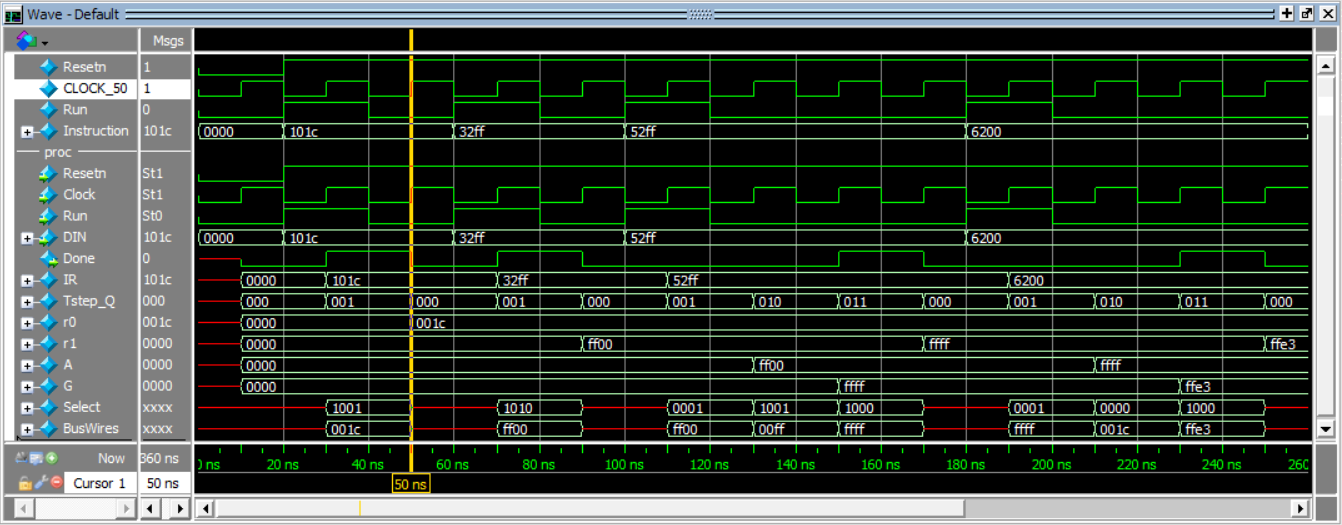
\includegraphics[scale=1.0]{figures/figure3.png}
	\end{center}
	\caption{Simulation results for the processor.}
	\label{fig:fig3}
\end{figure}
\section*{Part II}
\addcontentsline{toc}{2}{Part II}
In this part we will implement the circuit depicted in Figure~\ref{fig:fig4}, in which a 
memory module and counter are connected to the processor. The
counter is used to read the contents of successive locations in the memory, and
this data is provided to the processor as a stream of instructions. To simplify the
design and testing of this circuit we have used separate clock signals, {\it PClock} 
and {\it MClock}, for the processor and memory. Do the following:

\begin{enumerate}
\item A Quartus project file is provided along with this part of the exercise.  Use the 
Quartus software to open this project, which is called {\it part2.qpf}.
\item A sample top-level Verilog file that instantiates the processor, memory module, and
counter is shown in Figure~\ref{fig:procmem}. This code is provided in a file named
{\it part2.v}; it is the top-level file for the Quartus project {\it part2.qpf}. The 
code instantiates a memory module called {\it inst\_mem}. You have to create a Verilog file
that represents this memory module by using the Quartus software, as described below.

~\\
\begin{figure}[H]
	\begin{center}
		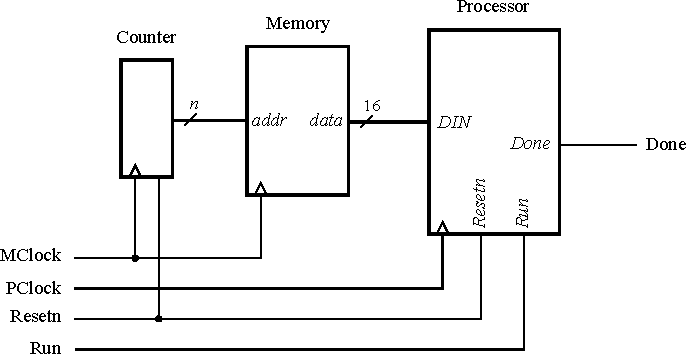
\includegraphics[]{figures/figure4.pdf}
	\end{center}
	\caption{Connecting the processor to a memory module and counter.}
	\label{fig:fig4}
\end{figure}
\newpage
\lstset{language=Verilog,numbers=none,escapechar=|}
\begin{figure}[h]
\begin{center}
\begin{minipage}[t]{12.5 cm}
\begin{lstlisting}[name=proc]
|\label{line:module}|
module part2 (KEY, SW, LEDR);
    input [1:0] KEY;
    input [9:0] SW;
    output [9:0] LEDR;	

    wire Done, Resetn, PClock, MClock, Run;
    wire [15:0] DIN;
    wire [4:0] pc;

    assign Resetn = SW[0];
    assign MClock = KEY[0];
    assign PClock = KEY[1];
    assign Run = SW[9];

    proc U1 (DIN, Resetn, PClock, Run, Done);
    assign LEDR[9] = Done;

    inst_mem U2 (pc, MClock, DIN);
    count5 U3 (Resetn, MClock, pc);
endmodule

module count5 (Resetn, Clock, Q);
    input Resetn, Clock;
    output reg [4:0] Q;

    always @ (posedge Clock, negedge Resetn)
        if (Resetn == 0)
            Q <= 5'b00000;
        else
            Q <= Q + 1'b1;
endmodule
\end{lstlisting}
\end{minipage}
\caption{Verilog code for the top-level module.}
\label{fig:procmem}
\end{center}
\end{figure}

\item
A diagram of the memory module that you need to create is depicted in Figure~\ref{fig:fig_ROM}.
Since this memory module has only a read port, and no write port, it is called a {\it synchronous 
read-only memory (synchronous ROM)}. Note that the memory module includes a register for 
synchronously loading addresses. This register is required due to the design of the memory 
resources in the Intel FPGA chip. 

Use the Quartus IP Catalog tool to create the memory module, by clicking on 
{\sf Tools} $>$ {\sf IP Catalog} in the Quartus software. In the IP Catalog window 
choose the {\it ROM:~1-PORT} module,
which is found under the {\sf Basic Functions $>$  On Chip Memory} category.  
Select {\sf Verilog HDL} as the type of output file to create, and give the file the name 
{\it inst\_mem.v}.

Follow through the provided dialogue to create a memory that has one 16-bit 
wide read data port and is 32 words deep. Figures~\ref{fig:fig5} and ~\ref{fig:fig6} show the 
relevant pages and how to properly configure the memory. 

\begin{figure}[t]
	\begin{center}
		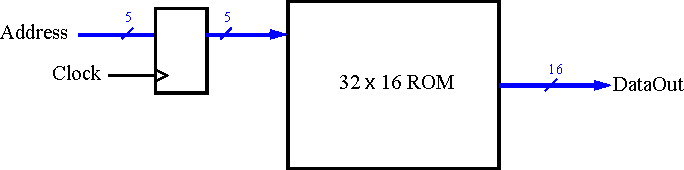
\includegraphics[]{figures/figure_ROM.pdf}
	\end{center}
	\caption{The 32 {\sf x} 16 ROM with address register.}
	\label{fig:fig_ROM}
\end{figure}

\begin{figure}[H]
	\begin{center}
		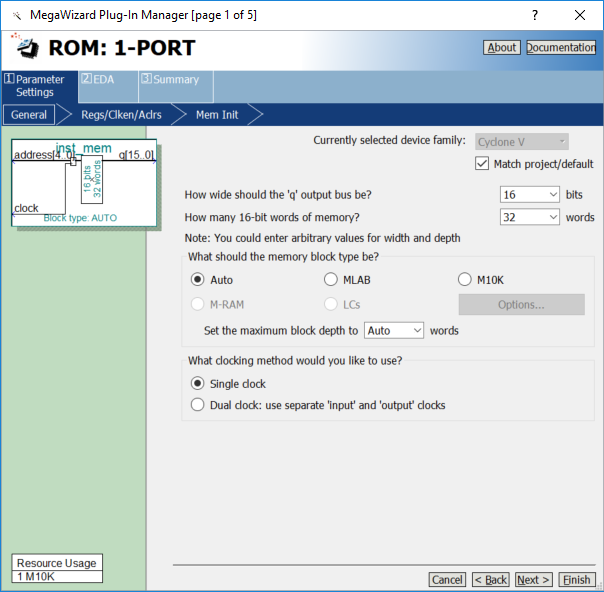
\includegraphics[scale=1.0]{figures/figure5.png}
	\end{center}
	\caption{{Specifying memory size.}}
	\label{fig:fig5}
\end{figure}

To place processor instructions into the memory, you need to specify {\it initial values}
that should be stored in the memory when your circuit is programmed into the FPGA chip.
This can be done by initializing the memory using the contents of a {\it memory initialization 
file (MIF)}. The appropriate screen is illustrated in Figure~\ref{fig:fig7}. We have specified 
a file named {\it inst\_mem.mif}, which then has to be created in the folder that 
contains the Quartus project. Clicking \texttt{Next} two more times will advance to the
\texttt{Summary} screen, which lists the names of files that will be created for the memory IP.
You should select {\it only} the Verilog file {\it inst\_mem.v}. Make sure that none of the 
other types of files are selected, and then click \texttt{Finish}.

An example of a memory initialization file is given in 
Figure~\ref{fig:fig_MIF}. Note that comments (\% $\ldots$ \%) are included in this file as a way of
documenting the meaning of the provided instructions.  Set the contents of
your {\it MIF} file such that it provides enough processor instructions to test your circuit.

\item The code in Figure~\ref{fig:procmem}, and the Quartus project, includes the necessary 
port names and pin location assignments to implement the circuit on a DE-series board.
The switch {\it SW}$_{9}$ drives the processor's {\it Run} input, {\it SW}$_0$ is
connected to {\it Resetn}, {\it KEY}$_0$ to {\it MClock}, and {\it KEY}$_1$ to {\it PClock}.
The Run signal is displayed on {\it LEDR}$_{0}$ and {\it Done} is connected to {\it LEDR}$_{9}$.
\begin{figure}[H]
	\begin{center}
		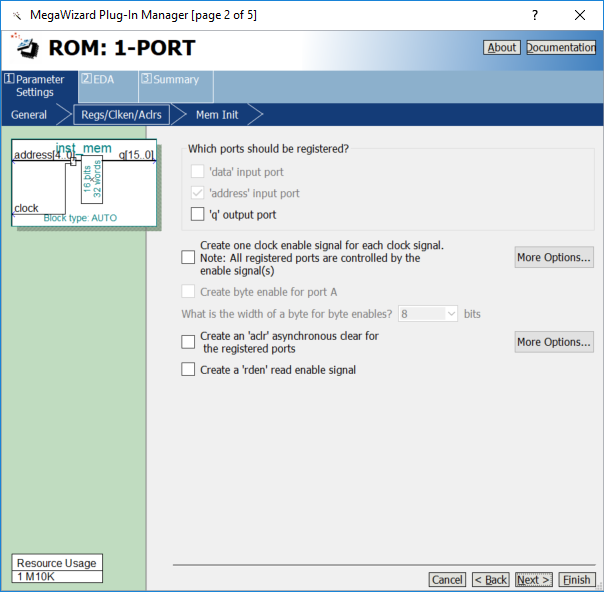
\includegraphics[scale=1.0]{figures/figure6.png}
	\end{center}
	\caption{Specifying which memory ports are registered.}
	\label{fig:fig6}
\end{figure}

\begin{figure}[H]
	\begin{center}
		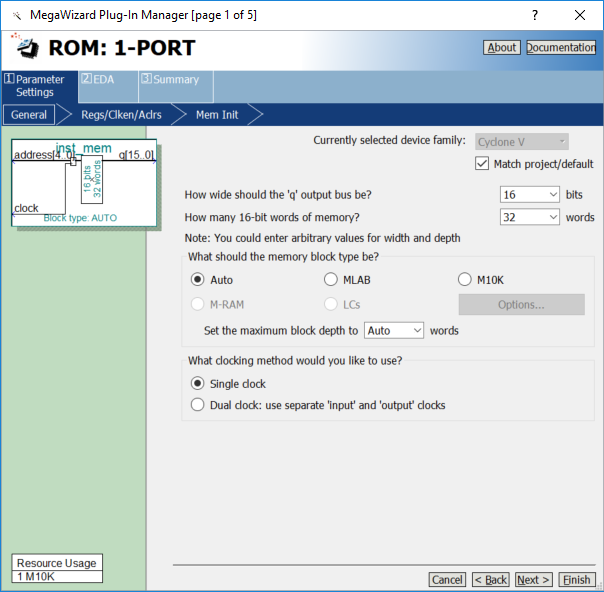
\includegraphics[scale=1.0]{figures/figure7.png}
	\end{center}
	\caption{Specifying a memory initialization file (MIF).}
	\label{fig:fig7}
\end{figure}

\item Use the ModelSim Simulator to test your Verilog code. Ensure 
that instructions are read properly out of the ROM and executed by the processor. An example 
of simulation results produced using ModelSim with the MIF file from 
Figure~\ref{fig:fig_MIF} is shown in Figure~\ref{fig:fig_sim2}. The corresponding ModelSim 
setup files are provided along with this exercise.
\item Once your simulations show a properly-working circuit, you may wish to download
it into a DE-series board. The functionality of the circuit on the board can be tested by
toggling the switches and observing the LEDs. Since the circuit's clock inputs are controlled 
by pushbutton switches, it is possible to step through the execution of instructions and 
observe the behavior of the circuit.
\end{enumerate}

\begin{figure}[H]
\begin{center}
\begin{minipage}[t]{12.5 cm}
\begin{tabbing}
{\bf DEPTH} = 32;\\
{\bf WIDTH} = 16;\\
{\bf ADDRESS\_RADIX} = HEX;\\
{\bf DATA\_RADIX} = BIN;\\
{\bf CONTENT}\\
{\bf BEGIN}\\
00	:	0001000000011100;~~~~~~\=\%~~mv  \=r0, \#0xFF00~~\=\% \kill
00	:	0001000000011100;	\>\% mv \>r0, \#28\>\%\\
01	:	0011001011111111; \>\% mvt \>r1, \#0xFF00\>\%\\
02	:	0101001011111111;	\>\% add  \>r1, \#0xFF\>\%\\
03	:	0110001000000000;	\>\% sub  \>r1, r0\>\%\\
04	:	0101001000000001;	\>\% add  \>r1, \#1\>\%\\
05	:	0000000000000000;\\
$\ldots$ (some lines not shown)\\
1F :	0000000000000000;\\
{\bf END};
\end{tabbing}
\end{minipage}
\end{center}
\caption{An example memory initialization file (MIF).}
\label{fig:fig_MIF}
\end{figure}

\begin{figure}[H]
	\begin{center}
		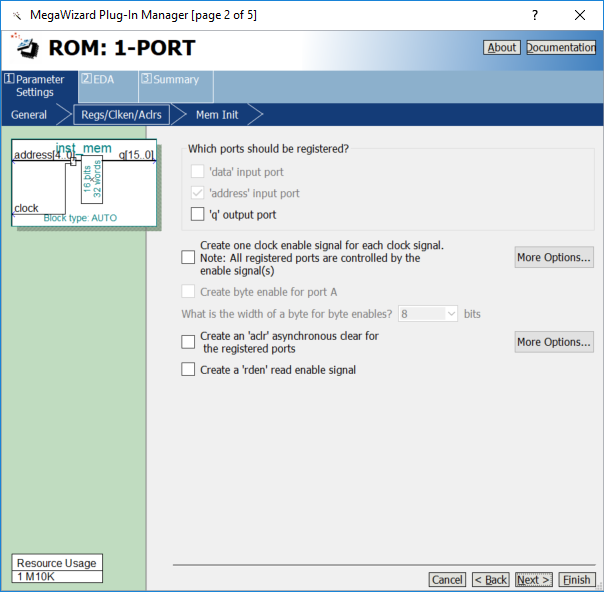
\includegraphics[scale=1.0]{figures/figure8.png}
	\end{center}
	\caption{An example simulation output using the MIF in Figure~\ref{fig:fig_MIF}.}
	\label{fig:fig_sim2}
\end{figure}

\section*{Enhanced Processor}
\addcontentsline{toc}{3}{Enhanced Processor}
It is possible to enhance the capability of the processor so that the counter in 
Figure~\ref{fig:fig4} is no longer needed, and so that the processor has the ability to 
perform read and write operations using memory or other devices. These enhancements involve 
adding new instructions to the processor, as well as other capabilities---they are
discussed in the next lab exercise.

\end{document}
